\newpage
\section{Ergebnisse, Diskussion und Ausblick}

In der durchgeführten Arbeit hat sich gezeigt, dass mit einer relativ kleinen Modifikation eine Implementierung von gemessenen Verzeichnungen realer Objektive in den vorhandenen Source Code von \textit{pbrt} implementiert werden konnte. Die einzige Schwierigkeit bestand darin, eine Invertierung der gemessenen Verzerrung zu bilden, welche numerisch errechnet werden musste. 

Anschließend konnten die damit durchgeführten Verzerrungen, wie sie exemplarisch in Abbildung \ref{fig:Guitar} an einem gerenderten Gitarren-Griffbrett zu sehen sind, mit einer bereits vorhandenen Matlab Implementierung verifiziert werden, wobei die Unterschiede der beiden Ergebnisse sich auf Ungenauigkeiten aufgrund von Interpolation zurückführen lassen.


\begin{figure}[h]
	\begin{subfigure}{.5\textwidth}
		\raggedleft
		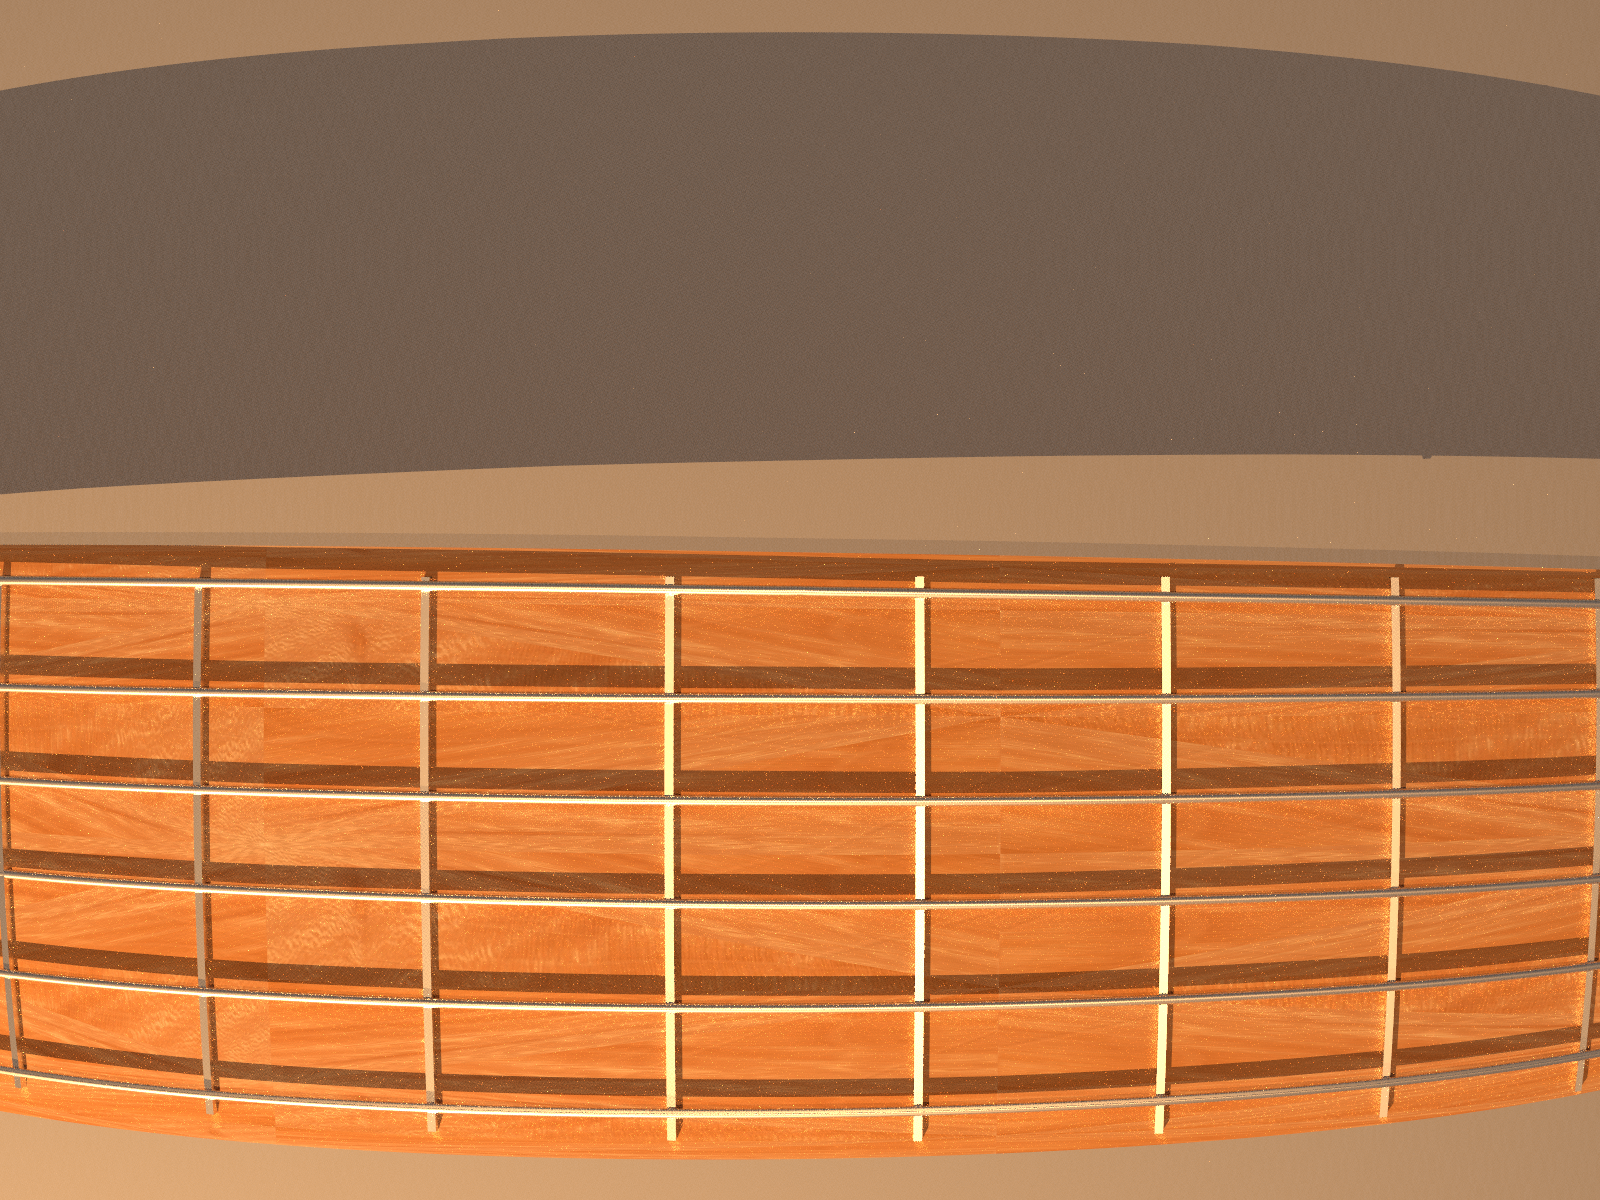
\includegraphics[width=\textwidth]{img/guitarDistorted.png}
		\caption{Poly3-Modell und $k=0.2$}
	\end{subfigure}
\begin{subfigure}{.5\textwidth}
		\raggedright
		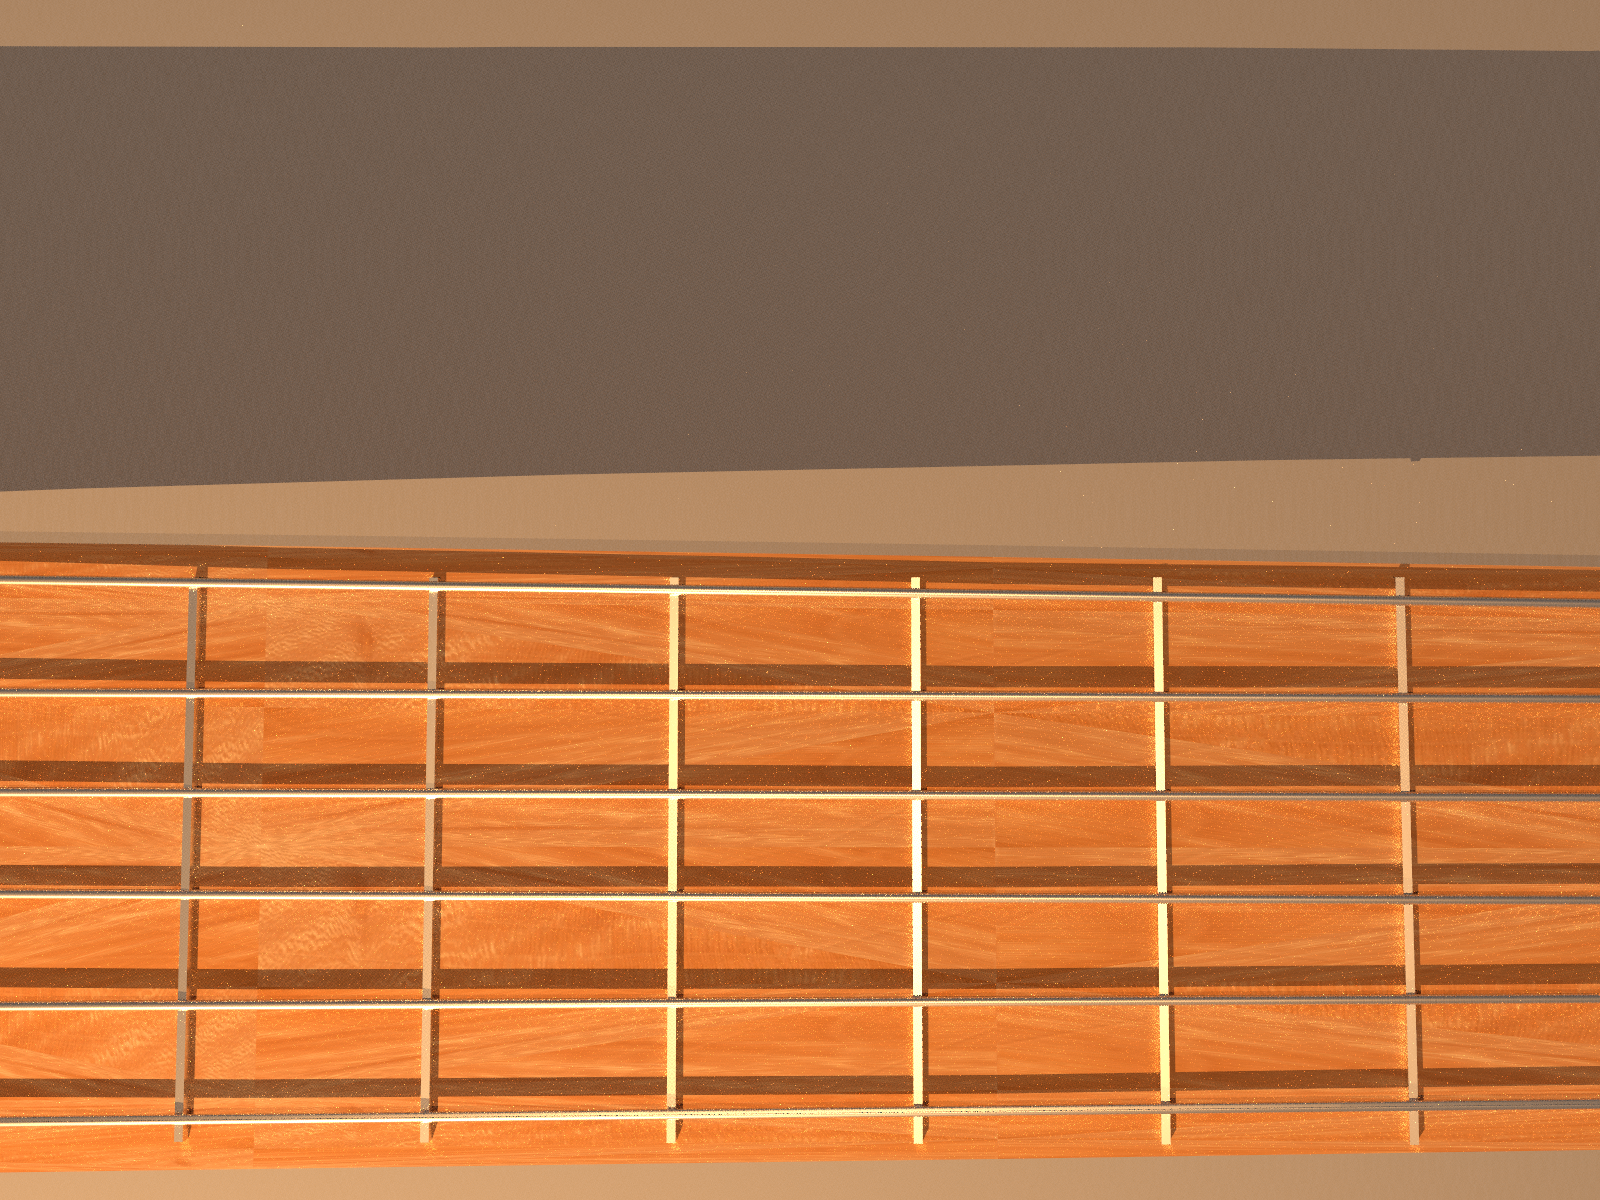
\includegraphics[width=\textwidth, ]{img/guitarUndist.png}
		\caption{Unverzerrt mit perspectiv camera}
	\end{subfigure}
\caption{Gerendertes Gitarrengriffbrett}
\label{fig:Guitar}
\end{figure}

Mögliche Erweiterungen der hier durchgeführten Implementierung könnten eine Verzerrung nach einem nicht radialsymmetrischen Modell umfassen. Auch wenn sich die meisten Verzeichnungen von Objektiven mit den hier genutzten Modellen gut abbilden lassen, liegt in der Realität nicht unbedingt eine komplett radialsymmetrische Verzerrung vor. So kann ein größere Genauigkeit durch ein getrenntes Abbilden der Verzerrung für x- und y-Richtung oder hinzufügen einer Tangentialkomponente zur Radialverzerrung erreicht werden. Auch das momentan in der Alpha Version von Lensfun integrierte Verzerrungsmodell nach Adobe Vorgaben kann integriert werden, wenn dessen Implementierung ausreichend getestet ist. 

Als weiteren Ausblick kann außerdem die Implementierung von Randabdunklungseffekten (Vignettierung) integriert werden, um eine weitere in der Realität auftretende Eigenschaft von Optiken zu berücksichtigen. 